\chapter{Implementácia}
\label{implementation}
V tejto kapitole podrobne popíšeme implementáciu podla návrhu v predchádzajúcej kapitole. Riešenie sme sa snažili spraviť dostatočne robustne na jednoduché rozširovanie v miestach pravdepodobných na zmenu správania v budúcnosti. Ale zároveň udržať nízku komplexitu a nevytvárať zbytočné vrstvy abstrakcie. Taktiež dodržiavať zaužívané princípy ako napríklad SOLID. 
Používali sme OOP ale aj funkcionálnu paradigmu a postupovali sme iteratívne. 

\begin{figure}[!ht]
    \centering
    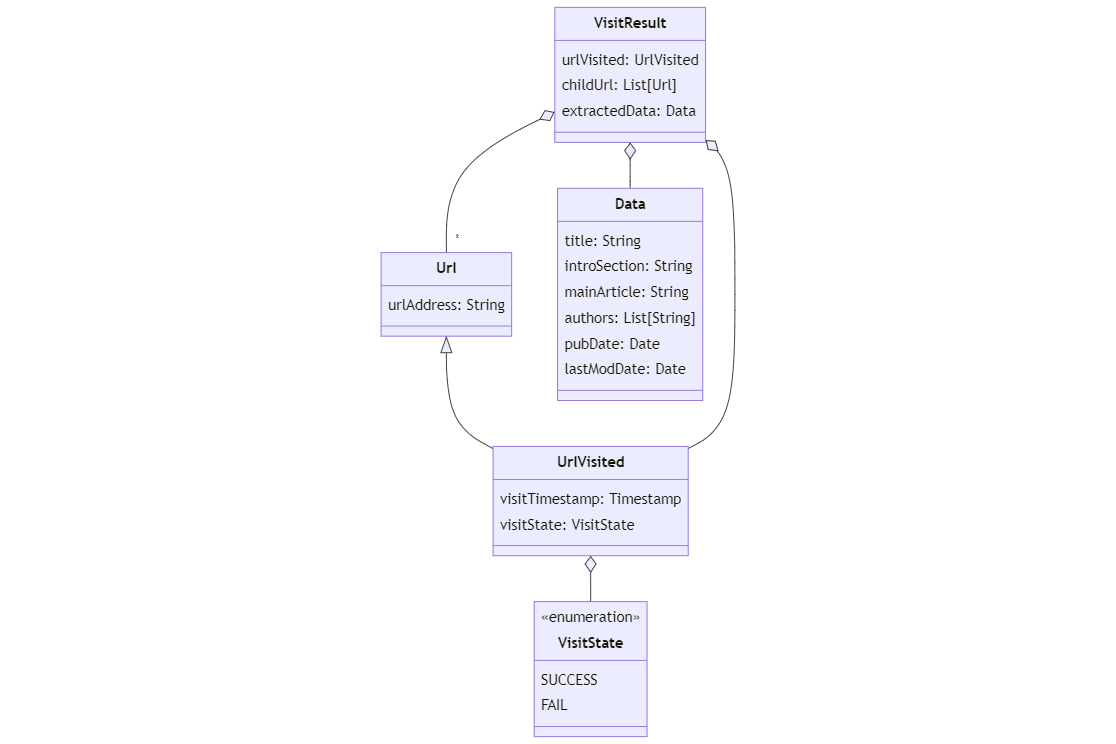
\includegraphics[width=.9\textwidth]{figures/classDiagramVisitResult.png}
    \caption{Class diagram pomocných dátových štruktúr \label{o:classDiagramVisitResult}}
\end{figure}

\section{Implementácia modulov}
V návrhu architektúry sme rozdelili riešenie do 4 základných modulov a popísali ich zodpovednosť a základnú komunikáciu medzi nimi. Taktiež sme popísali prístup k paralelizácii. V tejto podkapitole na to nadviažeme a popíšeme ako sme tieto moduly implementovali. 

\subsection{Orchestrátor}
Tento modul je vlastne jadro aplikácie, integrujúci zvyšné moduly. Tie komunikujú výlučne s ním a nie medzi sebou. Táto separácia nám umožnila jednoduché testovanie jednotlivých modulov a sledovanie komunikácie medzi nimi.

V implementácii sme nepoužili priamo pojem orchestrátor, ale implementovali sme ho v triede Crawler. Tá reprezentuje celú našu aplikáciu a jej metóda \textit{crawlMainJob} \todo{Ako pomenuvavat metody, oznacit ze ide o nazvy z kodu} štartuje samotný crawling. 

Pre jej inicializáciu musíme dodať objekt triedy CrawlerContext, obaľujúci inštancie zvyšných modulov. Takto vieme spúšťať crawler s rôznymi implementáciami modulov a tým meniť jeho správanie. Ide vlastne o známy princíp injektovania závislostí (dependency injection). \todo{Ak treba popisat benefity}

Po spustení sa vykonáva krok crowlovania, implementovaný funkciou doStep. Čo sa vykonáva v kroku je popísané v návrhu. Za zmienku ale stojí, že rozdelenie práce pracovným vláknam a agregovanie výsledku je presunuté do funkcie crawlStep. Tá pre pole adries vráti objekt CrawlResult. Bližšie si jej implementáciu popíšeme v samostatnej podkapitole. 

Návratovou hodnotou doStep je trieda RunStats. Tú priebežne agregujeme do CrawlerRunReport. Ide napríklad o počet navštívených adries a počet nezdarov. Využili sme triedy ako BigInt, kedže rátame s dlhodobým behom. 

\subsection{Funkcia crawlStep}
Táto funkcia rozdelí poskytnuté adresy parametrom do skupín. Každá skupina je potom spracovaná jedným z pracovných vlákien. Počet skupín je v štandardnom nastavení väčší ako počet pracovných vlákien. Tým zvýšime vyrovnanosť záťaže jednotlivých vlákien.

Využili sme abstrakciu nad paralelným spracovaním - \textit{Future}. Ide o generickú triedu štandardnej scala knižnice reprezentujúca budúcu hodnotu. V našom prípade budúcu hodnotu CrawlResult. Z pohľadu funkcionálneho programovanie je to monád. Tento prístup sa stáva populárnym aj v nie plno funkcionálnych programovacích jazykoch ako Java, Python a podobne. 

Práca vlákna je reprezentovaná funkciou crawlChunk. Tá mapuje skupinu adries na budúcu hodnotu CrawlResult. 

Funkcia crawlStep čaká na všetky budúce hodnoty, následne agreguje čiastkové výsledky práce do jedného. Reprezentujúceho výsledok navštívenia a extrahovania stránok určených na spracovanie v tomto kroku. 

Teda všetká paralelná činnosť programu je izolovaná v tejto funkcii. 

\subsection{Repozitár}
Modul repozitár reprezentuje interface s jednou metódou - saveStep. Jej jediný parameter je pole objektov RepoDTO (Data Transfer Objekt). Tento objekt reprezentuje schému ukladaných dát a je nezávislý na reprezentácií týchto dát vo zvyšku programu - PageResult. 

Táto striktná nezávislosť nám umožní v budúcnosti zmeniť spôsob ukladania výsledkov napríklad do relačnej databázy bez zásahu do zvyšku programu. Vytvoríme iba novú implementáciu tohto interfacu a vložíme ju do objektu CrawlerContext. 

Vytvorili sme 2 základné implementácie a jednú určenú na testovanie. Prvá ukladá výsledky všetkých krokov do jedného CSV súboru. To je vhodné pre krátke behy hlavne pri optimalizácii parametrov. Druhá ukladá každý krok do samostatného CSV. Pre produkčné nasadenie používame druhú implementáciu. 

Implementácia určená na testovanie ukladá objekty RepoDTO iba do vnútorného poľa. A pridáva metódu getAllSaved. To využívame v integračných testoch. Takto vieme skontrolovať či sa ukladajú do repozitára požadované výsledky a nemusíme pozerať do súborového systému. 


\subsection{Url Manažér}
Tento modul je reprezentovaný interfacom s metódami:
\begin{itemize}
    \item Upsert pridá Url adresy na prejdenie v budúcich krokoch. 
    \item GetBatch vráti adresy na prejdenie v aktuálnom kroku. 
    \item markAsCrawled označí adresy ako prejdené
\end{itemize}


Pri návrhu sme sa obávali, že nám uchovanie v operačnej pamäti nebude stačiť a budeme nútený použiť databázu. Ale testovanie aplikácie nepotvrdili túto obavu. Teda pre zníženie náročnosti na údržbu a infraštruktúru sme sa rozhodli pre jednoduchšie riešenie.

Hlavná implementácia tohto modulu ukladá potrebné dáta v operačnej pamäti a po každom volaní metód upsert a markAsCrawled je serializovaná na disk. Ako sme spomínali v návrhovej časti práce, zodpovednosťou tohto modulu je uchovanie stavu aj napriek pádom. 


Riešenie je pripravené na rozšírenie. V prípade potreby stačí implementovať tento modul robustnejšie a vložiť ho do CrawlerContext. 

\subsection{Extraktor}
Extraktor je implementovaný funkciou crawlUrl. Tá využíva interface DomainScraper s metódami na extrahovanie dát z html  dokumentu (parseDocument) a rozhodnutia či adresa je v danej doméne. Výsledkom extrahovania dát zo stránky je objekt PageContent. 

Následne funkcia crawlUrl odfiltruje podporované dcérske adresy pomocou triedy DomainFilter. Tie spolu s ďalšími hodnotami vráti v objekte CrawlResult. 

Crawled obsahuje teda iba pole podporovaných adries. PageContent na druhú stranu obsahuje všetky adresy nájdené na stránke. 

Pre pridanie podpory extrahovania z novej domény je potrebné implementovať DomainScraper a túto implementáciu pridať do zoznamu podporovaných domén. 


\section{Využitie parciálnej aplikácie funkcií vyššieho rádu}
Parciálna aplikácia je technika funkcionálneho programovania na zvýšenie znovu použiteľnosti funkcií, čitateľnosti a v našom prípade hlavne injektovania závislostí. Funkcia vyššieho rádu je funkcia berúca inú funkciu ako parameter alebo ako návratovú hodnotu. 

My sme tieto techniky využili hlavne pre injektovanie extraktora. Tento modul sme implementovali ako funkciu crawlUrl. Tá mapuje url na CrawlResult. Potrebuje získať html zo servera a extrahovať z neho relevantné dáta. 

Pre neprodukčné účely ako napríklad testovanie je pripájanie na server nežiadúce a chceme deterministickú implementáciu tejto funkcie. Tú vieme podsunúť ako parameter funkcii vyššieho rádu crawlChunk a crawlStep. Bližšie to popíšeme v podkapitole o testovní crawlera. 

\section{Zastavenie crawlera} \label{c:stopCrawling}
Za zastavenie crawlera mimo vyčerpania prehľadávanej fronty je zodpovedný interface CrawlLimit s metódou: shouldStopCrawling. Imeplementáciu poskytneme crawleru pri jeho inicializácii, takto vieme meniť podmienky zastavenia bez zásahu do kódu crawlera. Vytvorili sme 3 implementácie: 

\begin{itemize}
    \item StepLimitedCrawl - limitujeme počtom krokov.
    \item TimeLimitedCrawl - limitujeme ubehnutým časom od inicializácie, zastavíme crawlovanie až po skončení posledného kroku. 
    \item InfiniteCrawl - crawlovanie bez limitu.
\end{itemize}


\section{Testovanie}
Vďaka vhodnej architektúre môžeme každý modul mimo orchestrátora otestovať zvlášť. A orchestrátor otestovať spomínaným injektovaním závislostí. Takto poskytneme testovacie implementácie modulov pre izolované testovanie orchestrátora. Využívame jednotkové testy (unit tests). 

Integračnými testami testujeme hlavný scenár crolowania, teda či všetky moduly spolu komunikujú korektne. 

Beh crawlera je riadený odpoveďami zo serverov. Ak chceme vytvoriť deterministické testy nezávislé na vonkajšom prostredí, musíme tieto odpovede nahradiť. Posunuli sme to kúsok ďalej a nahrádzame celý extractor. Teda priradenie CrawlResult zadanej adrese. Práve na to sme využili spomínané parciálne aplikovanie funkcii vyššieho rádu.

Takto vieme vytvárať testovacie scenáre jednoducho, rýchlo a bez potreby písania html súborov. Stačí nám pre každý test vytvoriť funkciu priraďujúcu CrawlResult zadanej adrese. Príklad takejto funkcie uvádzame nižšie. Týmto spôsobom otestujeme takmer celú aplikáciu.

\begin{lstlisting}
    (u: Url) => u match {
        case "aaaa" => CrawlResult().addCrawled(crawled1)
        case "bbbb" => CrawlResult().addCrawled(crawled2)
        case "xxx" => CrawlResult().addFailed(Failed(u, "Url not supported"))
      }
\end{lstlisting}


Extraktor testujeme zvlášť na zopár pripravených HTML súboroch. Taktiež zopár testov sa priamo pripája na servery. Je ich malý počet a vieme ich spúšťať samostatne od hlavných testov. Teda zredukovali sme nezávislosť testov na minimum. 

GEnericke testy - \todo{popisat ako som spravil dedicnost v testoch aby nove implementacie url manazera nemuseli nanovo pisat testy. }

\section{Logovanie} \label{c:impl:logging}
Veľkú pozornosť sme kládli na dôkladné logovanie. Rátame s niekoľkohodinovým až pár dňovým behom aplikácie. V prípade pádu programu alebo nájdenia chyby potrebujeme čo najviac informácii pre diagnostiku.

Ako základ sme využili vstavanú Java knižnicu určenú a rozšírili sme ju o zápar, pre nás užitočných funkcionalít. Pridali sme napríklad meranie času od posledného zápisu. Takto sme priamo v zázname videli ubehnuté sekundy od minulého kroku. To môžeme vidieť na obrázku \ref{o:logExample} na riadku 32.

Taktiež sme vytvorili generickú funkciu s oddialeným vyhodnotením výrazov pre pohodlné meranie a zápis dĺžky behu častí programu. To sme využili pri odhaľovaní miest degradácie výkonu pri dlhých behoch. V príklade nižšie môžeme vidieť použitie tejto funkcie, nazvanej logTimedExp. 

\begin{lstlisting}
    logTimedExp("Getting Batch"){ctx.urlManager.getBatch(stepMaxSize)}
\end{lstlisting}

Výraz v zložených zátvorkách, zodpovedný za získanie adries, je vyhodnotený až v tele funkcie logTimedExp. Na obrázku \ref{o:logExample} na riadku 16 môžeme vidieť začiatok merania a na riadku 17 môžeme vidieť príslušný výpis s dĺžkou behu tohto výrazu. 

\begin{figure}[!ht]
    \centering
    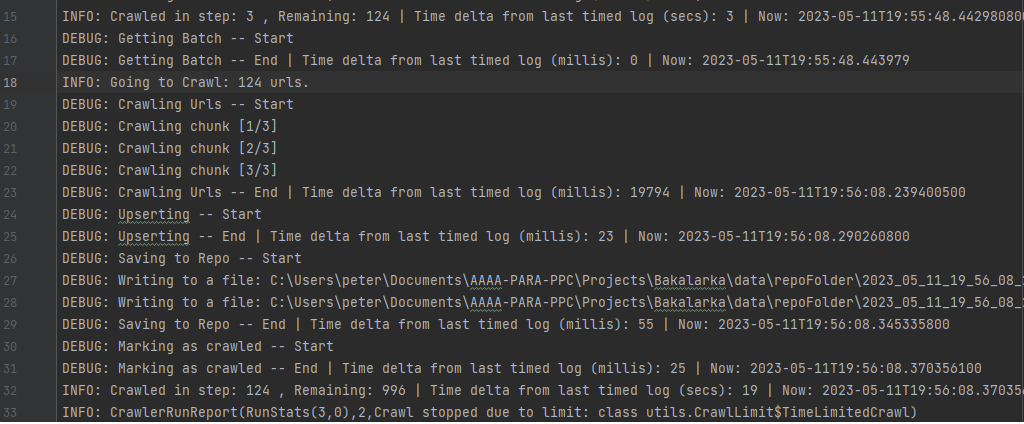
\includegraphics[width=1\textwidth]{figures/logExample.png}
    \caption{Príklad záznamov z behu crawlera}
    \label{o:logExample}
\end{figure}

\section{Inicializácia crawlera}
Z návrhu predpokladáme, že užívateľom bude človek s programátorkými schopnosťami a zmeny logiky extrakcie budú pomerne časté. Vytvorenie používateľského rozhrania preto považujeme za zbytočne vynaložené úsilie a rozhodli sme sa upravovať správanie crawlera priamo v kóde. Vytvorili sme vhodnú abstrakciu a úpravu v miestach, ktoré sme v návrhu označili sa potencionálne miesta rozširovania. Vytvorili sme sadu integračných a unit testov, na verifikovanie korektného nastavenia crawlera. 

Ako sme spomínali, objekt triedy CrawlerContext obaľuje hlavné moduly. Pomocou neho vieme injektovať závislosti. Napríklad ak v budúcnosti vznikne potreba ukladať zozbierané dáta do relačnej databázy, stačí vytvoriť novú implementáciu repozitára splňujúci kontrakt určený interfacom Repository. Inicializovať s ním CrawlerContext. Takto modifikujeme správanie crawlera bez priameho zásahu do jadra jeho kódu. Samozrejme je vhodné napísať unit testy pre novú implementáciu a spustiť s ňou aj už napísané integračné testy. Príklad inicializácie kontextu môžete vidieť na obrázku \ref{o:initCrawl} na riadku 26 až 30.

Ako sme popísali v analýze, ďalším dôležitým prvkom pre štart prehladávania je sada štartovacích adries nazývaných seeds. Pri jej volení sa snažíme vybrať aspoň jednu adresu z každého komponentu grafu odkazov. Čo môže byť problém, keďže tento graf dopredu nepoznáme. Inicializovanie tejto sady môžete vidieť na obrázku \ref{o:initCrawl} na riadku 33 až 37.

Dôležitou súčasťou nastavení je aj veľkosť kroku (stepMaxSize), udávajúca počet adries spracovaných v jednom kroku. Jej zvýšením vieme zefektívniť beh programu, keďže redukujeme počet neparalelných úsekov a prístup do súborového systému. Na druhú stranu ale zvyšujeme nároky na pamäť, keďže v nej pred uložením držíme práve tento počet výsledkov extrahovania. Teda ak zvolíme tento parameter príliš vysoký, program môže vyčerpať pridelenú operačnú pamäť. Oproti tomu menším problémom je aj zväčšenie veľkosti stratených dát pri páde programu. 

Dôležitou súčasťou nastavení je aj podmienka ukončenia crawlovanie. Na obrázku \ref{o:initCrawl} na riadku 43, je využitý časový zastavovač crawlera s využitím scala doménovo špecifického jazyka na reprezentáciu časového úseku. 


\begin{figure}[!ht]
    \centering
    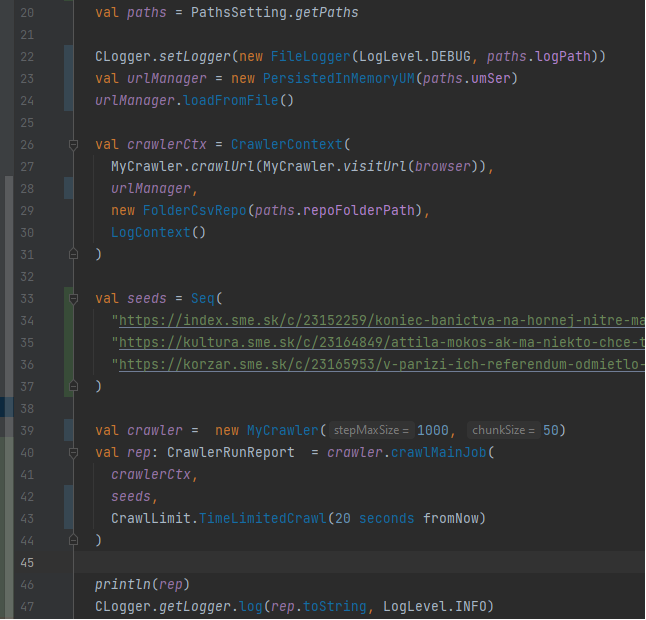
\includegraphics[width=.9\textwidth]{figures/crawlInit.png}
    \caption{Príklad inicializácie crawlera}
    \label{o:initCrawl}
\end{figure}

\section{Výzvy ktorým sme čelili pri implementácii riešenia}

\subsection{Nevhodný návrh tried reprezentujúcich výsledok.}
Prvá implementácia využívala polymorfizmus pre rozdielne správanie tried Crawled a Failed. Napríklad pri zápise do repozitára, alebo pri agregovaní štatistík. 

To ale spravilo tieto triedy zodpovednými za veľkú časť funkcionality crawlera. Čo je výrazné porušenie prvého zo zaužívaných SOLID princípov. Princíp jednej zodpovednosti (Single responsibility principle) hovorí, že každý modul by mal mať iba jeden dôvod na zmenu. V našom prípade by sa tieto triedy museli meniť so zmenou v agregovaní štatistík, zmenou v logike výberu adries na prechádzanie v jednom kroku, zmenou vo formáte alebo spôsobe ukladanie výsledkov. Teda takmer pri každej zmene na ktorú bola aplikácia navrhnutá. Čo je samozrejme veľmi nevhodný dizajn vedúci k zhoršenej udržiavateľnosti, testovateľnosti a spomaleniu rýchlosti vývoja.  

Preto sme sa rozhodli prerobiť aplikáciu a využiť kompozíciu na miesto dedičnosti. Čo nám umožnilo lepšie oddelenie zodpovedností. Z týchto tried sa stali iba jednoduché nosiče informácii bez logiky. Tá sa presunula do príslušných modulov.

\subsection{Vyčerpanie pamäte}
Pri návrhu sme predpokladali, že zozbieraná dáta sú väčšie ako dostupná operačná pamäť. Preto agregujeme a ukladáme výsledky pracovných vlákien pravidelne. 

Prvá verzia, slúžiaca len na demonštráciu funkčnosti návrhu, agregovala aj čiastkové výsledky a po konci crolowanie z nich vypočítala štatistiky. Napríklad percentuálnu úspešnosť extrakcie. 

Pri vytváraní finálnej implementácie sme to neodstránili a pri nasadení nám to po necelej hodine padlo. Z výpisu chyby vyplývalo, že pamäť sa minula pri zápise do modulu manažujúceho adresy (UrlManager). V spojení s obavami opísaných pri návrhu sme vyčerpanie pamäte pripisovali práve tomuto modulu. Až analýza použitia pamäte nás nasmerovala k zabudnutému kódu. 

Ten sme nahradili priebežným počítaním štatistík. 